\subsubsection*{Obteniendo el valor máximo}
%El problema de la mochila analiza, 
	%Un problema no analiza nada, los algoritmos lo hacen
% para cada objeto, el máximo valor que se puede obtener para cada capacidad posible de la mochila. Si llamamos $K$ a la capacidad de la mochila, se evaluará introducir un elemento $e$ en la capacidad $k$ con 1 $\leq$ $k$ $\leq$ $K$. 

Si tenemos una sola mochila, nuestro algoritmo analiza para cada objeto el máximo valor que se puede obtener para cada capacidad posible de la mochila. Es decir, que si llamamos $K$ a la capacidad total de la mochila y a $k$ un numero entero con 1 $\leq$ $k$ $\leq$ $K$, entonces para todos los $k$ se evaluará introducir un elemento $e$ en la capacidad posible $k$.

%En cada evaluación se decide entre no meter el elemento, con lo cual el valor máximo de la mochila que tenga la capacidad $k$ será el calculado con algún elemento anterior (o cero en el caso de que sea el primero en ser evaluado); o meter el elemento, con lo cual, al valor del elemento se le suma el valor de la mochila de capacidad k - $peso(e)$ que sea máxima. De esta forma, se genera un subproblema que respeta el principio de optimalidad, con lo cual se puede aplicar programación dinámica para solucionar el problema. \\


En cada evaluación se decide si me llevo el elemento en la mochila o no. Dado el caso:

\begin{itemize}
	\item Decido no meter el elemento: Se calcula el valor máximo de la mochila que tenga la capacidad $k$ será el calculado solamente usando elementos anteriores. El valor será cero si no hay elementos anteriores o no es posible insertarlos en esa capacidad.
	\item Decido meter el elemento en la mochila: Al valor del elemento se le suma el valor máximo de la mochila de capacidad k - $peso(e)$ y eso resulta en el valor máximo de la mochila con capacidad $k$.
\end{itemize} 

%TODO creo que lo del principio de optimalidad no iba no?
 De esta forma, se genera un subproblema que respeta el principio de optimalidad, con lo cual se puede aplicar programación dinámica para solucionar el problema. \\ 
 
%Extendiendonos a 2 mochilas, al evaluar la $k$ posibilidad de la primer mochila (con capacidad $K_{a}$), 
	% de donde sale el a
% se debe tener en cuenta que tambien está la posibilidad de utilizar la segunda mochila (con capacidad $K_{b}$).
	% de donde sale b
	% definimos mochila a y b o aprovechando que dijimos primera y segunda uso k1 y k2 
	%Los graficos de Esteban usan numeros tambien
% Esto nos muestra que por cada elemento debemos calcular $K_{a} \times K_{b}$ combinaciones de capacidades. Sin contar el primer elemento, 
	%por que   
%el resto calculará sus combinaciones en base a las del elemento que le precedió en la evaluación, siguiendo la idea del algoritmo original de una mochila. Para obtener el valor final, se buscará en la matriz resultante de evaluar el último elemento, a la combinación de capacidades entre ambas mochilas que resulte máxima.\\
 	%Ok habia una matriz, como que sale de la nada, antes de este parrafo convendria explicar las estructuras? O abstraer un poco y hablar de eso mas tarde?

  En el caso de 2 mochilas, al evaluar la $k$ posibilidad de la primer mochila (con capacidad $k_{1}$), se debe tener en cuenta que tambien está la posibilidad de utilizar la segunda mochila (con capacidad $k_{2}$). Esto nos muestra que por cada elemento debemos calcular $k_{1} \times k_{2}$ combinaciones de capacidades. Siguiendo la idea del algoritmo original para una mochila, se calcularán sus combinaciones en base a las del elemento que le precedió en la evaluación. Para obtener el valor definitivo, luego de evaluar hasta el último elemento se selecciona la combinación de capacidades entre ambas mochilas que resulte máxima.\\
 
%TODO me gustaria explicar el subproblema de la programacion dinamica más al principio y de una mejor manera
Como explicamos antes, ibamos a resolver este problema mediante programación dinámica. Esto quiere decir que necesitamos almacenar resultados de subproblemas previamente calculados. Nuestro subproblema es hallar el valor maximo para la suma de los valores de los objetos para un subconjunto de los elementos y con ciertas capacidades en las mochilas.
%no menciono la cantidad de mochilas porque no es una variable. Una vez comienza el algoritmo es una constante para todos los subproblemas
Siendo $M$ la cantidad de mochilas disponibles, debemos poseer una matriz de $M$ dimensiones para cada objeto, permitiendo así guardar un valor máximo para cada combinación posible de capacidades de las mochilas.

  \vspace*{0.3cm} \vspace*{0.3cm}
  \begin{center}
 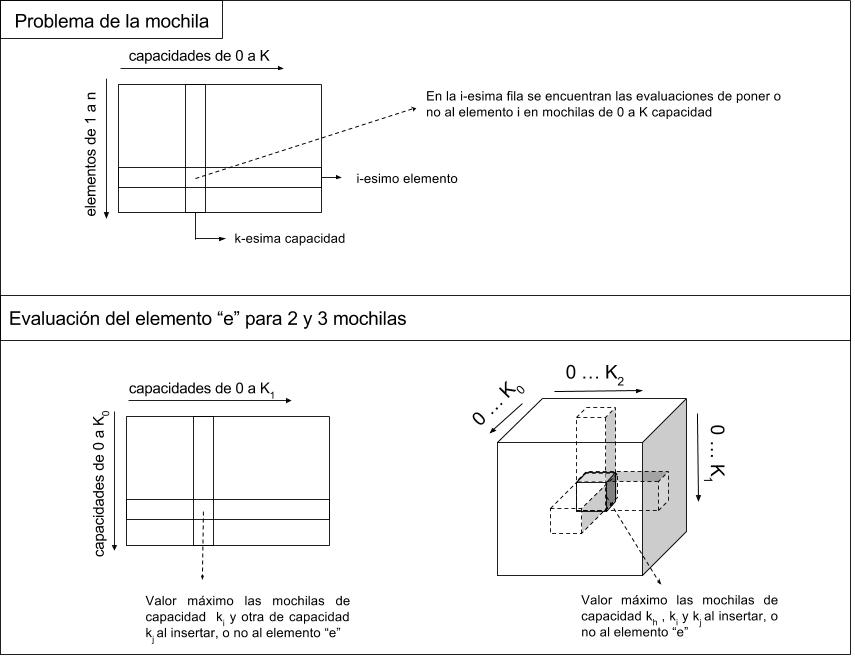
\includegraphics[scale=0.6]{./EJ3/dibujo-matrices.jpg}
  \end{center}
  \vspace*{0.3cm}
  
  Con la misma lógica podemos ver que para 3 mochilas donde se tienen capacidades  $K_{1}$,$K_{2}$ y $K_{3}$, cada elemento disponible evaluará $K_{1} \times K_{2} \times K_{3}$ posibilidades. En este caso se buscará la solución en la matriz tridimensional de posibilidades obtenidas del último elemento evaluado.


\subsubsection*{Recuperando los elementos utilizados}

Siendo que la consigna pide los objetos involucrados en la solución, es necesaria una forma de, a partir de los valores máximos obtenidos, deducir los elementos que fueron usados y el lugar donde fueron colocados para lograr el resultado.\\
%Buena introduccion

%Analizando la última matriz del caso de 2 mochilas (sin perder generalización para 3 mochilas), 
	%no me suena bien lo del parentesis
	%tiene sentido aclarar para dos mochilas? Lo usamos mas adelante a ese hecho?
%podemos notar que por cada objeto que iteramos para intentar encontrarle un lugar en las mochilas, deja el valor previo, de cada combinacion de capacidades, sin tocar cuando el objeto no es utilizado. Al ser utilizado, se cambia el valor por el nuevo máximo alcanzado.  
	%Me cuesta entender esto
%De utilizar 1 matriz solamente, y actualizarla por cada objeto, se perderá la posibilidad de saber si se usó o no a cada uno, ya que no se tendrá un "paso anterior" por haber sido reescrito en cada paso subsiguiente. \\
	

Analizando la última matriz del caso de 2 mochilas (sin pérdida de generalidad para 3 mochilas). 

Por cada objeto iterado, notamos las siguientes posibilidades en una celda especifica de su matriz:

\begin{itemize}
	\item Si el objeto no es utilizado en ese caso, el valor de la celda es igual al valor de la celda correspondiente en la matriz del objeto anterior.
	\item Si el objeto es utilizado, el valor de la celda es un nuevo maximo alcanzado. Por lo tanto el valor de la celda del objeto actual difiere (y en particular, es mayor) con el valor correspondiente al objeto anterior.
	%Es mayor no?
\end{itemize}

De utilizar 1 matriz solamente, y actualizarla por cada objeto, se perderá la posibilidad de saber si se usó o no a cada uno, ya que no se tendrá un "paso anterior" por haber sido reescrito en cada paso subsiguiente. \\


Para recuperar estos estados, se resuelve guardar la matriz involucrada en el c\'alculo de cada elemento. Llamando a las matrices del elemento i M, y N a la del elemento j subsiguiente a i (ambas de dimensión $K_{a} \times K_{b}$), se tiene que si el maximo se encuentra en $N_{yz}$ y es igual a $M_{yz}$, entonces quiere decir que el algoritmo al evaluar la posibilidad de meter al elemento j en esa combinación, opto por excluirlo, con lo cual no es perteneciente a la solución final. Si en cambio el valor es superior, indica que el valor guardado en la instancia M fue incrementado, y usado a j en la solución.\\
%No me gusta mucho. Siento que se repiten varias veces las cosas

Finalmente, para saber en que mochila fue introducido cada elemento, se busca en la instancia M, mochila a cuya capacidad se le restó el peso $p(j)$ de j. Esto lo podemos saber cuando el valor de $N_{yz} = M_{(y-p(j),z)}$ en el caso de que se encuentre en la mochila "a" o $N_{yz} = M_{(y,z-p(j))}$ en caso contrario.\\
%Calculo que no hay demasiadas formas más copadas de decir esto

  \vspace*{0.3cm} \vspace*{0.3cm}
  \begin{center}
 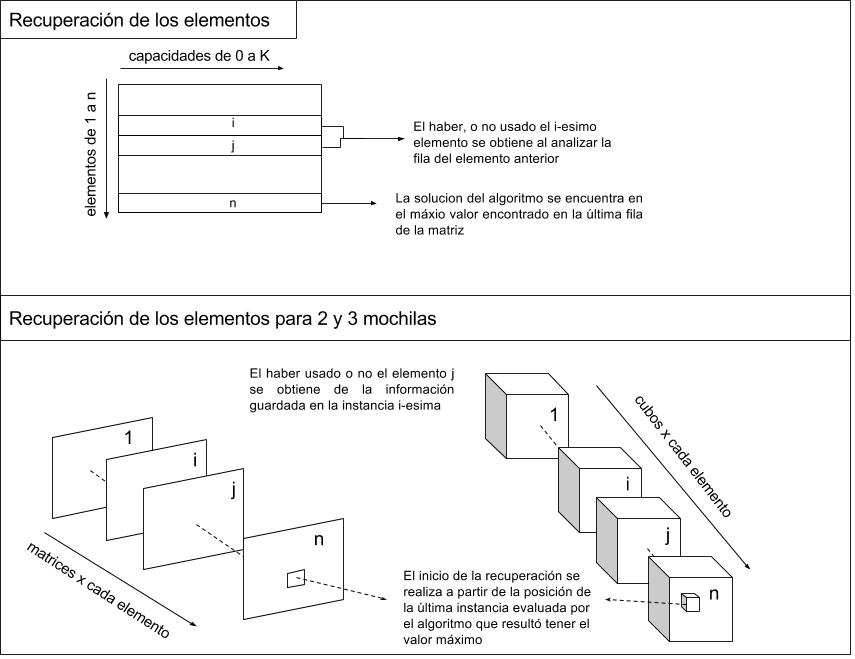
\includegraphics[scale=0.6]{./EJ3/dibujo-recuperacion.jpg}
  \end{center}
  \vspace*{0.3cm}

 Para el caso de 3 mochilas, no se pierde generalidad: En vez de contar con matrices bidimensionales se utilizan tridimensionales, y se compara $N_{xyz} = M_{(x-p(j),y,z)}$, $N_{xyz} = M_{(x,y-p(j),z)}$, $N_{xyz} = M_{(x,y,z-p(j))}$ para determinar la pertenencia de cada objeto a la solución.
%Si lo analizo un poco capaz que encuentro una forma de decir esto en lenguaje natural 
 